\documentclass[../main/Notes.tex]{subfiles}
\begin{document}

\newcommand{\cfbox}[2]{%
    \colorlet{currentcolor}{.}%
    {\color{#1}%
    \fbox{\color{currentcolor}#2}}%
}

\section[Solution 6: Signal Detection Theory xxxBut which number to put here?xxx]{Solution 6: Signal Detection Theory I+II \iftoggle{showdates}{\small{\textit{2014-06-27}}}{}}

\subsection*{Excercise 4}\index{Low Threshold Theory}\label{sheet6ex4}

Luce's idea is: If High Threshold Theory does not work, maybe by using a low threshold, ROC curves will be explainable. This idea translates as follows:

\begin{align*}
S \in \{ y,n \} , D \in \{ y,n \} , R \in \{ y,n \} \\
P\left(D=y|S=y\right) = p_{y} \\
P\left(D=y|S=n\right) = p_{n} > 0
\end{align*}

We have to consider to different cases of the subject's behaviour.

\textbf{Case 1:} The subject want to lower his false-alarm rate $p(FA)$:
\begin{align*}
& P\left(R=y|D=n\right) = 0 \\
& P\left(R=y|D=y\right) = t < 1\\
\Rightarrow P(FA) & = P\left(R=y|D=y\right) &\cdot~& P\left(D=y|S=n\right) &+~&P\left(R=y|D=n\right)&\cdot~ & P\left(D=n|S=n\right) \\
& = t &\cdot~& p_{n} &+~& 0 &\cdot~& \left(1-p_{n}\right) \\
& = t \cdot~ p_{n} \\
\Rightarrow P(H) & = P\left(R=y|D=y\right) &\cdot~& P\left(D=y|S=y\right) &+~&P\left(R=y|D=n\right)&\cdot~ & P\left(D=n|S=y\right) \\
& = t &\cdot~& p_{y} &+~& 0 &\cdot~& \left(1-p_{y}\right) \\
& = t \cdot~ p_{y} \\
& = \frac{P(FA)}{p_{n}} \cdot~ p_{y}
\end{align*}

Now the first part of the plot looks like this:
\begin{figure}[ht!]
  \centering
  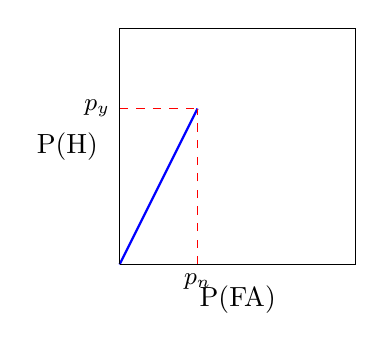
\begin{tikzpicture}[scale=3]
  \node[below] at (0.33,0) {\small $p_{n}$};
  \node[left] at (0,0.66) {\small $p_{y}$};
    \node[below] at (0.5,-0.05) {P(FA)};
  \node[left] at (-0.05,0.5) {P(H)};
  \draw[thick, blue] (0,0) -- (0.33,0.66);
  \draw[dashed, red] (0.33,0) -- (0.33,0.66);
   \draw[dashed, red] (0,0.66) -- (0.33,0.66);
   	\draw (0,0) -- (0,1) --(1,1) -- (1,0) -- (0,0);
  \end{tikzpicture}
  \caption{Low Threshold Model, first part of plot with slope of $\frac{p_{y}}{p_{n}}$}
  \label{fig:2014-06-27_firstPartLowThrsh}
\end{figure}

\textbf{Case 2:} The subject wants a higher hit rate $p(H)$:
\begin{align*}
& P\left(R=y|D=Y\right) = 1 \\
& P\left(R=y|D=n\right) = u > 0\\
\Rightarrow P(FA) & = P\left(R=y|D=y\right) &\cdot~& P\left(D=y|S=n\right) &+~&P\left(R=y|D=n\right)&\cdot~ & P\left(D=n|S=n\right) \\
& = 1 &\cdot~& p_{n} &+~& u &\cdot~& \left(1-p_{n}\right) \\
& = p_{n} + u \cdot~ \left(1-p_{n}\right)\\
\Leftrightarrow u &= \frac{P(FA)-p_{n}}{1-p_{n}} \\
\Rightarrow P(H) & = P\left(R=y|D=y\right) &\cdot~& P\left(D=y|S=y\right) &+~&P\left(R=y|D=n\right)&\cdot~ & P\left(D=n|S=y\right) \\
& = 1 &\cdot~& p_{y} &+~& u &\cdot~& \left(1-p_{y}\right) \\
& = p_{y} +  u \cdot~  \left(1-p_{y}\right)\\
& = p_{y} +  \frac{P(FA)-p_{n}}{1-p_{n}} \cdot~  \left( 1-p_{y} \right)\\
& = \frac{1-p_{y}}{1-p_{n}} \cdot~ P(FA) + \frac{p_{y}-p_{n}}{1-p_{n}}
\end{align*}

We can finish our plot:
\begin{figure}[ht!]
  \centering
  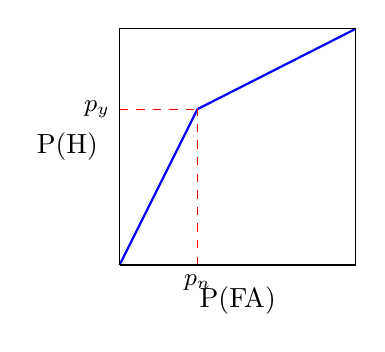
\begin{tikzpicture}[scale=3]
  \node[below] at (0.33,0) {\small $p_{n}$};
  \node[left] at (0,0.66) {\small $p_{y}$};
    \node[below] at (0.5,-0.05) {P(FA)};
  \node[left] at (-0.05,0.5) {P(H)};
  \draw[thick, blue] (0,0) -- (0.33,0.66);
   \draw[thick, blue] (0.33,0.66) -- (1,1);
  \draw[dashed, red] (0.33,0) -- (0.33,0.66);
   \draw[dashed, red] (0,0.66) -- (0.33,0.66);
   	\draw (0,0) -- (0,1) --(1,1) -- (1,0) -- (0,0);
  \end{tikzpicture}
  \caption{Low Threshold Model Plot}
  \label{fig:2014-06-27_LowThrshPlot}
\end{figure}

As can be seen, Low Threshold Theory better fits the actual data since its form is, compared with the linear function of High Threshold Theory, more like that of an ROC curve. Nevertheless it is not the right model for what is really going on.

\subsection*{Excercise 5}\index{ROC Curve}\label{sheet6ex5}

\begin{figure}[ht!]
\begin{minipage}{.25\textwidth}
  \centering
  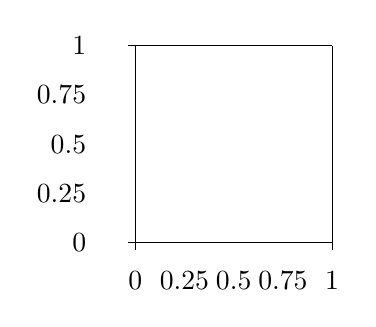
\begin{tikzpicture}[scale=2.5]
  % ticks horizontal
  \foreach \x in {0,...,1}
    \draw (\x,1pt) -- (\x,-1pt);
  % labels horizontal
  \draw	(0,-0.1) node[anchor=north] {0}
		    (0.25,-0.1) node[anchor=north] {0.25}
		    (0.5,-0.1) node[anchor=north] {0.5}
		    (0.75,-0.1) node[anchor=north] {0.75}
		    (1,-0.1) node[anchor=north] {1}
        ;
  
 % ticks vertical
  \foreach \y in {0,...,1}
    \draw (1pt, \y) -- (-1pt, \y);
  % labels vertical
  \draw (-0.2,0.0) node[anchor=east]  {0}
        (-0.2,0.25) node[anchor=east]  {0.25}
        (-0.2,0.5) node[anchor=east]  {0.5}
        (-0.2,0.75) node[anchor=east]  {0.75}
        (-0.2,1) node[anchor=east] {1}
        ;
  
  \draw[green,thick] plot[smooth] file {../data/2014-06-27_plot1.txt};
    \draw[green,thick] plot[smooth] file {../data/2014-06-27_plot1_2.txt};
%  \draw (0.30854,0.69146) circle (1cm);

    % axis square
  \draw[-] (0, 0) -- (1, 0);
  \draw[-] (0, 0) -- (0, 1);
  \draw[-] (0, 1) -- (1, 1);
  \draw[-] (1, 0) -- (1, 1);  
    \end{tikzpicture}
  \caption{\small One datapoint of a Signal Detection Experiment}
  \label{fig:2014-06-27_exe5_1}
  \end{minipage}
  \cfbox{white}{
  \vspace{0.125\textwidth} }
%\end{figure}
%\begin{figure}[ht!]
\begin{minipage}{.25\textwidth}
  \centering
  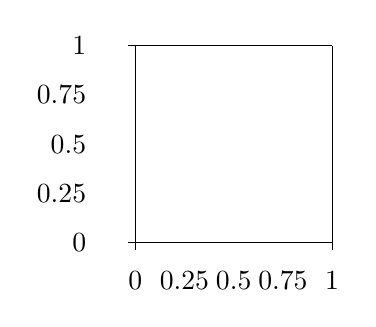
\begin{tikzpicture}[scale=2.5]
  % ticks horizontal
  \foreach \x in {0,...,1}
    \draw (\x,1pt) -- (\x,-1pt);
  % labels horizontal
  \draw	(0,-0.1) node[anchor=north] {0}
		    (0.25,-0.1) node[anchor=north] {0.25}
		    (0.5,-0.1) node[anchor=north] {0.5}
		    (0.75,-0.1) node[anchor=north] {0.75}
		    (1,-0.1) node[anchor=north] {1}
        ;
  
  % ticks vertical
  \foreach \y in {0,...,1}
    \draw (1pt, \y) -- (-1pt, \y);
  % labels vertical
  \draw (-0.2,0.0) node[anchor=east]  {0}
        (-0.2,0.25) node[anchor=east]  {0.25}
        (-0.2,0.5) node[anchor=east]  {0.5}
        (-0.2,0.75) node[anchor=east]  {0.75}
        (-0.2,1) node[anchor=east] {1}
        ;
  \draw[green,thick] plot[smooth] file {../data/2014-06-27_plot2.txt};

    % axis square
  \draw[-] (0, 0) -- (1, 0);
  \draw[-] (0, 0) -- (0, 1);
  \draw[-] (0, 1) -- (1, 1);
  \draw[-] (1, 0) -- (1, 1);  

%  \draw (0.30854,0.69146) circle (1cm);
    \end{tikzpicture}
  \caption{\small ROC curve with distance of gaussians d = 1}
  \label{fig:2014-06-27_exe5_2}
\end{minipage}
  \cfbox{white}{
  \vspace{0.125\textwidth} }
%\end{figure}
%\begin{figure}[ht!]
\begin{minipage}{.25\textwidth}
  \centering
  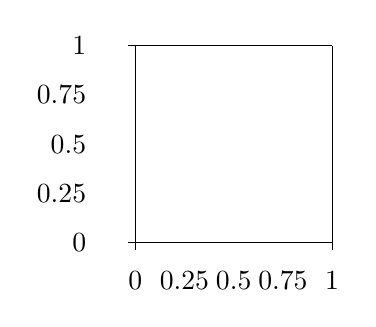
\begin{tikzpicture}[scale=2.5]
  % ticks horizontal
  \foreach \x in {0,...,1}
    \draw (\x,1pt) -- (\x,-1pt);
  % labels horizontal
  \draw	(0,-0.1) node[anchor=north] {0}
		    (0.25,-0.1) node[anchor=north] {0.25}
		    (0.5,-0.1) node[anchor=north] {0.5}
		    (0.75,-0.1) node[anchor=north] {0.75}
		    (1,-0.1) node[anchor=north] {1}
        ;
  
  % ticks vertical
  \foreach \y in {0,...,1}
    \draw (1pt, \y) -- (-1pt, \y);
  % labels vertical
  \draw (-0.2,0.0) node[anchor=east]  {0}
        (-0.2,0.25) node[anchor=east]  {0.25}
        (-0.2,0.5) node[anchor=east]  {0.5}
        (-0.2,0.75) node[anchor=east]  {0.75}
        (-0.2,1) node[anchor=east] {1}
        ;
  \draw[green,thick] plot[smooth] file {../data/2014-06-27_plot3.txt};

    % axis square
  \draw[-] (0, 0) -- (1, 0);
  \draw[-] (0, 0) -- (0, 1);
  \draw[-] (0, 1) -- (1, 1);
  \draw[-] (1, 0) -- (1, 1);  

%  \draw (0.30854,0.69146) circle (1cm);
    \end{tikzpicture}
  \caption{\small ROC curve with distance of gaussians d = 0}
  \label{fig:2014-06-27_exe5_3}
\end{minipage}
\end{figure}

\begin{figure}[ht!]
\begin{minipage}{.25\textwidth}
  \centering
  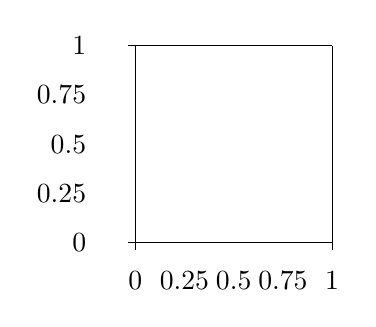
\begin{tikzpicture}[scale=2.5]
  % ticks horizontal
  \foreach \x in {0,...,1}
    \draw (\x,1pt) -- (\x,-1pt);
  % labels horizontal
  \draw	(0,-0.1) node[anchor=north] {0}
		    (0.25,-0.1) node[anchor=north] {0.25}
		    (0.5,-0.1) node[anchor=north] {0.5}
		    (0.75,-0.1) node[anchor=north] {0.75}
		    (1,-0.1) node[anchor=north] {1}
        ;
  
  % ticks vertical
  \foreach \y in {0,...,1}
    \draw (1pt, \y) -- (-1pt, \y);
  % labels vertical
  \draw (-0.2,0.0) node[anchor=east]  {0}
        (-0.2,0.25) node[anchor=east]  {0.25}
        (-0.2,0.5) node[anchor=east]  {0.5}
        (-0.2,0.75) node[anchor=east]  {0.75}
        (-0.2,1) node[anchor=east] {1}
        ;
  \draw[green,thick] plot[smooth] file {../data/2014-06-27_plot4.txt};

    % axis square
  \draw[-] (0, 0) -- (1, 0);
  \draw[-] (0, 0) -- (0, 1);
  \draw[-] (0, 1) -- (1, 1);
  \draw[-] (1, 0) -- (1, 1);  

%  \draw (0.30854,0.69146) circle (1cm);
    \end{tikzpicture}
  \caption{ROC curve with distance of gaussians d = 1/2}
  \label{fig:2014-06-27_exe5_4}
  \end{minipage}
%\end{figure}
\cfbox{white}{
  \vspace{0.125\textwidth} }
%\begin{figure}[ht!]
\begin{minipage}{.25\textwidth}  
  \centering
  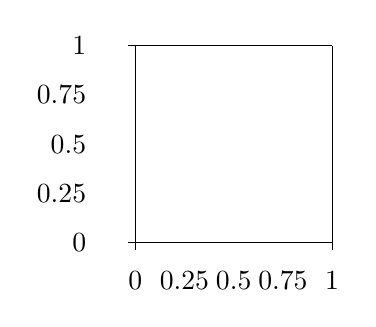
\begin{tikzpicture}[scale=2.5]
  % ticks horizontal
  \foreach \x in {0,...,1}
    \draw (\x,1pt) -- (\x,-1pt);
  % labels horizontal
  \draw	(0,-0.1) node[anchor=north] {0}
		    (0.25,-0.1) node[anchor=north] {0.25}
		    (0.5,-0.1) node[anchor=north] {0.5}
		    (0.75,-0.1) node[anchor=north] {0.75}
		    (1,-0.1) node[anchor=north] {1}
        ;
  
  % ticks vertical
  \foreach \y in {0,...,1}
    \draw (1pt, \y) -- (-1pt, \y);
  % labels vertical
  \draw (-0.2,0.0) node[anchor=east]  {0}
        (-0.2,0.25) node[anchor=east]  {0.25}
        (-0.2,0.5) node[anchor=east]  {0.5}
        (-0.2,0.75) node[anchor=east]  {0.75}
        (-0.2,1) node[anchor=east] {1}
        ;
  \draw[green,thick] plot[smooth] file {../data/2014-06-27_plot5.txt};

    % axis square
  \draw[-] (0, 0) -- (1, 0);
  \draw[-] (0, 0) -- (0, 1);
  \draw[-] (0, 1) -- (1, 1);
  \draw[-] (1, 0) -- (1, 1);  

%  \draw (0.30854,0.69146) circle (1cm);
    \end{tikzpicture}
  \caption{ROC curve with distance of gaussians d = 2}
  \label{fig:2014-06-27_exe5_5}
  \end{minipage}
%\end{figure}
\cfbox{white}{
  \vspace{0.125\textwidth} }
%\begin{figure}[ht!]
\begin{minipage}{.25\textwidth}
  \centering
  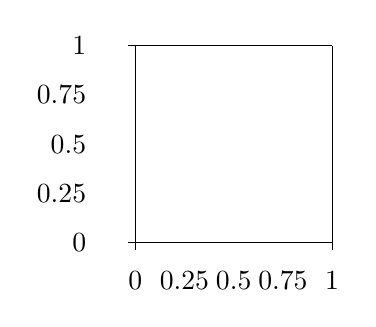
\begin{tikzpicture}[scale=2.5]
  % ticks horizontal
  \foreach \x in {0,...,1}
    \draw (\x,1pt) -- (\x,-1pt);
  % labels horizontal
  \draw	(0,-0.1) node[anchor=north] {0}
		    (0.25,-0.1) node[anchor=north] {0.25}
		    (0.5,-0.1) node[anchor=north] {0.5}
		    (0.75,-0.1) node[anchor=north] {0.75}
		    (1,-0.1) node[anchor=north] {1}
        ;
  
  % ticks vertical
  \foreach \y in {0,...,1}
    \draw (1pt, \y) -- (-1pt, \y);
  % labels vertical
  \draw (-0.2,0.0) node[anchor=east]  {0}
        (-0.2,0.25) node[anchor=east]  {0.25}
        (-0.2,0.5) node[anchor=east]  {0.5}
        (-0.2,0.75) node[anchor=east]  {0.75}
        (-0.2,1) node[anchor=east] {1}
        ;
  \draw[green,thick] plot[smooth] file {../data/2014-06-27_plot6.txt};

    % axis square
  \draw[-] (0, 0) -- (1, 0);
  \draw[-] (0, 0) -- (0, 1);
  \draw[-] (0, 1) -- (1, 1);
  \draw[-] (1, 0) -- (1, 1);  

%  \draw (0.30854,0.69146) circle (1cm);
    \end{tikzpicture}
  \caption{ROC curve with distance of gaussians d = 3}
  \label{fig:2014-06-27_exe5_6}
  \end{minipage}
\end{figure}
%PART TWO OF EXE5
%\begin{figure}[ht!]
\captionsetup{type=figure} 
\begin{minipage}{.25\textwidth}
  \centering
  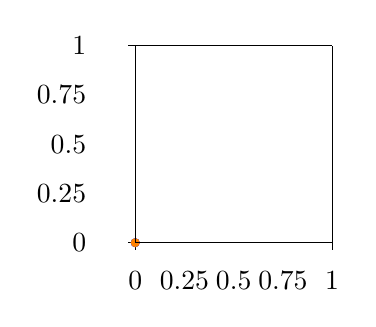
\begin{tikzpicture}[scale=2.5]
  % ticks horizontal
  \foreach \x in {0,...,1}
    \draw (\x,1pt) -- (\x,-1pt);
  % labels horizontal
  \draw	(0,-0.1) node[anchor=north] {0}
		    (0.25,-0.1) node[anchor=north] {0.25}
		    (0.5,-0.1) node[anchor=north] {0.5}
		    (0.75,-0.1) node[anchor=north] {0.75}
		    (1,-0.1) node[anchor=north] {1}
        ;
  
  % ticks vertical
  \foreach \y in {0,...,1}
    \draw (1pt, \y) -- (-1pt, \y);
  % labels vertical
  \draw (-0.2,0.0) node[anchor=east]  {0}
        (-0.2,0.25) node[anchor=east]  {0.25}
        (-0.2,0.5) node[anchor=east]  {0.5}
        (-0.2,0.75) node[anchor=east]  {0.75}
        (-0.2,1) node[anchor=east] {1}
        ;
  \draw[green] plot[smooth] file {../data/2014-06-27_plot7.txt};
  \draw[red,ultra thick] plot[smooth] file {../data/2014-06-27_plot_triangle_c1_1.txt} circle (0.3pt);
   \draw[blue,ultra thick] plot[smooth] file {../data/2014-06-27_plot_triangle_c1_2.txt} circle (0.3pt);
    \draw[yellow,ultra thick] plot[smooth] file {../data/2014-06-27_plot_triangle_c1_3.txt} circle (0.pt);
     \draw[magenta,ultra thick] plot[smooth] file {../data/2014-06-27_plot_triangle_c1_4.txt} circle (0.3pt);
    \draw[cyan,ultra thick] plot[smooth] file {../data/2014-06-27_plot_triangle_c1_5.txt} circle (0.3pt);     
    \draw[orange,ultra thick] plot[smooth] file {../data/2014-06-27_plot_triangle_c1_6.txt} circle (0.3pt);  
    % axis square
  \draw[-] (0, 0) -- (1, 0);
  \draw[-] (0, 0) -- (0, 1);
  \draw[-] (0, 1) -- (1, 1);
  \draw[-] (1, 0) -- (1, 1);  

%  \draw (0.30854,0.69146) circle (1cm);
    \end{tikzpicture}
  \caption{Subject with criterion c=1/4}
  \label{fig:2014-06-27_exe5_7}
  \end{minipage}
%\end{figure}
\cfbox{white}{
  \vspace{0.125\textwidth} }
%\begin{figure}[ht!]
\begin{minipage}{.25\textwidth}  
  \centering
  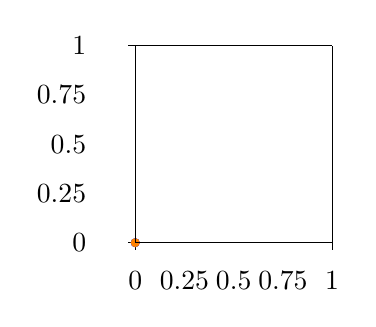
\begin{tikzpicture}[scale=2.5]
  % ticks horizontal
  \foreach \x in {0,...,1}
    \draw (\x,1pt) -- (\x,-1pt);
  % labels horizontal
  \draw	(0,-0.1) node[anchor=north] {0}
		    (0.25,-0.1) node[anchor=north] {0.25}
		    (0.5,-0.1) node[anchor=north] {0.5}
		    (0.75,-0.1) node[anchor=north] {0.75}
		    (1,-0.1) node[anchor=north] {1}
        ;
  
  % ticks vertical
  \foreach \y in {0,...,1}
    \draw (1pt, \y) -- (-1pt, \y);
  % labels vertical
  \draw (-0.2,0.0) node[anchor=east]  {0}
        (-0.2,0.25) node[anchor=east]  {0.25}
        (-0.2,0.5) node[anchor=east]  {0.5}
        (-0.2,0.75) node[anchor=east]  {0.75}
        (-0.2,1) node[anchor=east] {1}
        ;
  \draw[green] plot[smooth] file {../data/2014-06-27_plot8.txt};
  \draw[red,ultra thick] plot[smooth] file {../data/2014-06-27_plot_triangle_c2_1.txt} circle (0.3pt);
   \draw[blue,ultra thick] plot[smooth] file {../data/2014-06-27_plot_triangle_c2_2.txt} circle (0.3pt);
    \draw[yellow,ultra thick] plot[smooth] file {../data/2014-06-27_plot_triangle_c2_3.txt} circle (0.pt);
     \draw[magenta,ultra thick] plot[smooth] file {../data/2014-06-27_plot_triangle_c2_4.txt} circle (0.3pt);
    \draw[cyan,ultra thick] plot[smooth] file {../data/2014-06-27_plot_triangle_c2_5.txt} circle (0.3pt);     
    \draw[orange,ultra thick] plot[smooth] file {../data/2014-06-27_plot_triangle_c2_6.txt} circle (0.3pt);  
    % axis square
  \draw[-] (0, 0) -- (1, 0);
  \draw[-] (0, 0) -- (0, 1);
  \draw[-] (0, 1) -- (1, 1);
  \draw[-] (1, 0) -- (1, 1);  

%  \draw (0.30854,0.69146) circle (1cm);
    \end{tikzpicture}
  \caption{Subject with criterion c=1/2}
  \label{fig:2014-06-27_exe5_8}
  \end{minipage}
%\end{figure}
\cfbox{white}{
  \vspace{0.125\textwidth} }
%\begin{figure}[ht!]
\begin{minipage}{.25\textwidth}
  \centering
  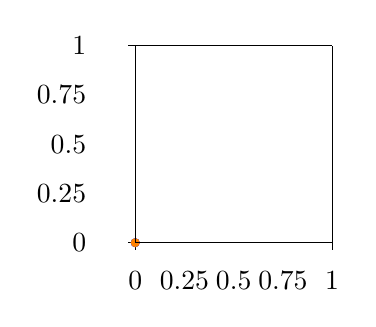
\begin{tikzpicture}[scale=2.5]
  % ticks horizontal
  \foreach \x in {0,...,1}
    \draw (\x,1pt) -- (\x,-1pt);
  % labels horizontal
  \draw	(0,-0.1) node[anchor=north] {0}
		    (0.25,-0.1) node[anchor=north] {0.25}
		    (0.5,-0.1) node[anchor=north] {0.5}
		    (0.75,-0.1) node[anchor=north] {0.75}
		    (1,-0.1) node[anchor=north] {1}
        ;
  
  % ticks vertical
  \foreach \y in {0,...,1}
    \draw (1pt, \y) -- (-1pt, \y);
  % labels vertical
  \draw (-0.2,0.0) node[anchor=east]  {0}
        (-0.2,0.25) node[anchor=east]  {0.25}
        (-0.2,0.5) node[anchor=east]  {0.5}
        (-0.2,0.75) node[anchor=east]  {0.75}
        (-0.2,1) node[anchor=east] {1}
        ;
  \draw[green] plot[smooth] file {../data/2014-06-27_plot9.txt};
  \draw[red,ultra thick] plot[smooth] file {../data/2014-06-27_plot_triangle_c3_1.txt} circle (0.3pt);
   \draw[blue,ultra thick] plot[smooth] file {../data/2014-06-27_plot_triangle_c3_2.txt} circle (0.3pt);
    \draw[yellow,ultra thick] plot[smooth] file {../data/2014-06-27_plot_triangle_c3_3.txt} circle (0.pt);
     \draw[magenta,ultra thick] plot[smooth] file {../data/2014-06-27_plot_triangle_c3_4.txt} circle (0.3pt);
    \draw[cyan,ultra thick] plot[smooth] file {../data/2014-06-27_plot_triangle_c3_5.txt} circle (0.3pt);     
    \draw[orange,ultra thick] plot[smooth] file {../data/2014-06-27_plot_triangle_c3_6.txt} circle (0.3pt);     

    % axis square
  \draw[-] (0, 0) -- (1, 0);
  \draw[-] (0, 0) -- (0, 1);
  \draw[-] (0, 1) -- (1, 1);
  \draw[-] (1, 0) -- (1, 1);  

%  \draw (0.30854,0.69146) circle (1cm);
    \end{tikzpicture}
  \caption{Subject with criterion c=3/2}
  \label{fig:2014-06-27_exe5_9}
  \end{minipage}
%\end{figure}
\hspace{1cm}
\\
\hspace{1cm}
\\
\hspace{1cm}
\\
\texttt{MATLAB} code for exercise 5:
\matlabcode{../data/sheet6_exe5.m}

\subsection*{Excercise 6}\index{Rating Data}\label{sheet6ex6}

Signal detection experiments are pretty extensive - 200 trials mean nothing at all. Before the experimenter has 15,000 trials it is not worth even starting (or so a wise man said).
Thus we can introduce a method that gives more data for each. To do this, we introduce a scale from 0 to 3, where 0 is absolutely not and 3 absolutely yes. It could look like this:

\captionsetup{type=figure} 
\begin{tikzpicture}
  \begin{axis}[domain=-1.25:2.5, enlargelimits=upper, axis x line*=bottom, axis y line*=left]

       \addplot+[domain=0.5:1.5, samples=50, pattern=north east lines, mark=none
                hatch distance=5pt, hatch thickness=0.5pt,
                draw=orange, pattern color=orange!40, forget plot]
                {gauss(0.25,0.35)} \closedcycle;
   \addplot+[domain=-1.25:0.25, samples=50, pattern=north east lines, mark=none
                hatch distance=5pt, hatch thickness=0.5pt,
                draw=red, pattern color=red!40, area legend]
                {gauss(0.25,0.35)} \closedcycle;
    \addlegendentry{say 0}
    
     \addplot+[domain=0.25:0.5, samples=50, pattern=north west lines, mark=none
                hatch distance=2pt, hatch thickness=0.5pt,
                draw=blue, pattern color=blue!40, area legend]
                {gauss(0.25,0.35)} \closedcycle;
    \addlegendentry{say 1}
           \addplot+[domain=0.5:1.5, samples=50, pattern=north east lines, mark=none
                hatch distance=5pt, hatch thickness=0.5pt,
                draw=orange, pattern color=orange!40, area legend]
                {gauss(1.5,0.35)} \closedcycle;
 \addlegendentry{say 2}
 
       \addplot+[domain=1.5:2.5, samples=50, pattern=north west lines, mark=none
                hatch distance=2pt, hatch thickness=0.5pt,
                draw=green, pattern color=green!40, area legend]
                {gauss(1.5,0.35)} \closedcycle;
    \addlegendentry{say 3}
    
    \addplot [dashed,samples=50]   {gauss(0.25,0.35)};
      \addlegendentry{noise};
    \addplot [samples=50] {gauss(1.5,0.35)};
      \addlegendentry{signal};
      
  \draw[blue,thick] (axis cs: 0.5,0) -- (axis cs: 0.5,1.65);           
        \draw[red, thick] (axis cs: 0.25,0) -- (axis cs: 0.25,1.65);
        \draw[green,thick] (axis cs: 1.5,0) -- (axis cs: 1.5,1.65);
  \end{axis}

\end{tikzpicture}
\caption{Gaussians with different criterions}
\label{fig:2014-06-27-exe6}
\sidenote{introducing a scale is a great idea, but be aware that more than 7 response categories are hard to handle by the subjects}
Now varying the range on the scale we count as an 'no'-response, we get more points for our ROC curve.\\
\textit{Example:} Take 0 as 'no', 1-3 as 'yes $\rightarrow$ plot this point\\
Take 0-1 as 'no', 2-3 as 'yes $\rightarrow$ plot this point\\
Take 0-2 as 'no', 3 as 'yes $\rightarrow$ plot this point
\end{document}